\documentclass[a4paper]{article}

\usepackage[utf8]{inputenc}
\usepackage[portuges]{babel}
\usepackage{graphicx}
\usepackage{a4wide}
\usepackage[pdftex]{hyperref}
\usepackage{float}
\usepackage{graphicx}
\usepackage{indentfirst}
\usepackage[small]{caption}


\begin{document}

\title{Projeto de Laboratórios de Informática III\\Grupo 1}
\author{Catarina Machado (a81047) \and Cecília Soares (a34900) \and João Vilaça (a82339)}
\date{\today}

\begin{titlepage}

  %título
  \thispagestyle{empty}
  \begin{center}
  \begin{minipage}{0.75\linewidth}
      \centering
  %engenharia logo
      
\includegraphics[width=0.4\textwidth]{eng.jpeg}\par\vspace{1cm}
      \vspace{1.5cm}
  %titulos
      \href{https://www.uminho.pt/PT}{\scshape\LARGE Universidade do Minho} \par
      \vspace{1cm}
      \href{https://www.di.uminho.pt/}{\scshape\Large Departamento de Informática} \par
      \vspace{1.5cm}

  \maketitle

  \end{minipage}
  \end{center}
  \clearpage

 \end{titlepage}


\begin{abstract}
O presente relatório descreve o projeto realizado no âmbito da disciplina de
\href{http://miei.di.uminho.pt/plano_estudos.html#laborat_rios_de_inform_tica_iii}
{\emph {Laboratórios de Informática III} (LI3)}, ao longo do segundo semestre,
do segundo ano, do \href{http://miei.di.uminho.pt}{Mestrado Integrado em Engenharia Informática}
da \href{https://www.uminho.pt}{Universidade do Minho}.

O objetivo do projeto foi desenvolver um sistema capaz de processar a informação
contida em ficheiros XML para responder a um conjunto de interrogações de forma
eficiente, utilizando, para isso, a linguagem de programação Java. Neste documento
descrevemos sucintamente o tipo concreto de dados e as estruturas de dados usadas,
a modularização funcional e abstração de dados a que recorremos, as estratégias seguidas
em cada uma das interrogações e as estratégias utilizadas para melhoramento de desempenho.

\end{abstract}
\pagebreak

\tableofcontents


\pagebreak

\section{Introdução}
\label{sec:intro}

O presente relatório foi elaborado no âmbito da unidade curricular
\href{http://miei.di.uminho.pt/plano_estudos.html#laborat_rios_de_inform_tica_iii}
{\emph {Laboratórios de Informática III} (LI3)}, ao longo do segundo semestre,
do segundo ano, do \href{http://miei.di.uminho.pt}{Mestrado Integrado em Engenharia Informática}
da \href{https://www.uminho.pt}{Universidade do Minho}, e tem como objetivo
descrever as tarefas desenvolvidas para criar um sistema capaz de processar as
informações contidas em ficheiros XML para responder a um conjunto de
interrogações de forma eficiente, utilizando a linguagem de programação Java.


\subsection{Descrição do Problema}
\label{sec:problema}

Os ficheiros em formato XML que deveriam ser processados continham informação referente ao
website \href{https://stackoverflow.com/}{\textit{Stack Overflow}}.

Em concreto, o trabalho prendia-se em extrair a informação necessária dos vários
ficheiros, de forma a conseguirmos responder a 11 interrogações relacionadas com
o conteúdo dos mesmos da forma mais eficiente possível, isto é, tendo especial
atenção ao tempo de execução do programa, ao encapsulamento dos dados, bem como
à modularização do código.

\subsection{Ficheiros XML}
\label{sec:xml}

De todos os ficheiros XML colocados à nossa disposição (Votes, Tags, Users,
PostLinks, Posts, PostHistory, Comments e Badges) e que se destinavam a dar resposta
a um conjunto de interrogações, decidimos que apenas iríamos precisar de carregar
algumas informações contidas nos ficheiros Tags.xml, Users.xml e Posts.xml. \par
Do ficheiro Tags.xml retiramos somente o identificador da tag (ID) e o nome da mesma
(TagName). Do ficheiro Users.xml, recolhemos a informação relativa ao identificador
do utilizador (ID), à sua reputação (Reputation), ao seu nome (DisplayName) e ao seu
perfil (AboutMe). \par
Por último, quanto ao ficheiro Posts.xml extraímos o identificador
do post (ID); o tipo de post (PostTypeId); o utilizador que publicou o post
(OwnerUserId); o título do post (Title); as suas tags (Tags); a pontuação obtida
(Score); o número de comentários que foram feitos (CommentCount); no caso de
ser uma resposta, o número da pergunta a que se refere (ParentId) e, finalmente,
a sua data de criação (CreationDate).

\subsection{Concepção da Solução}
\label{sec:solucao}

Para resolvermos este problema foram cruciais três momentos. Numa primeira fase,
definimos a estrutura de dados que consideramos que melhor solucionaria o nosso
problema. Posteriormente, analisamos as vantagens e desvantagens das diferentes
alternativas para fazer a leitura dos dados e a recolha da informação relevante.
A nossa opção recaiu na utilização da API SAX para fazer o \textit{parser} da
informação, dado que permite o acesso serial ao conteúdo de um documento XML de
forma orientada a eventos, aquilo a que chamam \textit{event-based parser} para
os documentos XML.
Finalmente, na última etapa do projeto concentramo-nos em responder
às diferentes \textit{queries}.

O código subjacente à solução proposta pode ser encontrado no repositório:

\begin{center}
\href{https://github.com/dium-li3/Grupo1}{\emph{https://github.com/dium-li3/Grupo1}}.
\end{center}

O restante deste relatório está organizado da seguinte forma: a
Secção~\ref{sec:estruturadedados} descreve as estruturas de dados adoptadas,
ao passo que a Secção~\ref{sec:implementacao}  apresenta e discute a solução
proposta para a resolução do problema. O relatório termina com conclusões na
Secção~\ref{sec:conclusao}, onde é também apresentada uma análise crítica dos
resultados obtidos.



\section{Organização dos Dados}
\label{sec:estruturadedados}

Para desenvolvermos este trabalho adotamos as seguintes estruturas de dados:

\subsection{Tipo de Dados Concretos}
\label{sec:dados_concretos}

\begin{verbatim}
public class TCD_Community implements TADCommunity {
    private Map<Long, Users> users;
    private Map<Long, Posts> posts;
    private Set<Question> questionsSet;
    private Set<Users> usersSet;
    private List<Long> usersPostList;
    private Map<LocalDate, Day> days;
    private Map<String, Long> tags;
\end{verbatim}

\vspace{0.2cm}

Os dados necessários para responder às queries foram armazenados
na classe \texttt{TCD\_Community}, que contém os apontadores para as principais
estruturas de dados do nosso trabalho, bem como os métodos necessários para aceder
a essa mesma classe de forma a garantir o encapsulamento dos dados.


Em primeiro lugar, \textbf{users}, \textbf{posts},
e \textbf{tags} utilizamos a interface map para armazenar os dados,
o que nos permite implementar quer uma HashMap quer uma TreeMap. \par
A razão para essa escolha deve-se ao facto de tantos os IDs dos users, como os
IDs das questions, answers e tags não estarem armazenados nos ficheiros de forma
sequencial, nem serem contíguos (existem ``buracos'' entre os respetivos números
identificadores), pelo que se utilizássemos os IDs como sendo os índices de um
array haveria muita memória desperdiçada, e, por isso, não vimos nenhuma vantagem
em utilizar as interfaces \textbf{List} ou \textbf{Queue}. \par
De facto, a nossa opção recaiu sobre a classe HashMap para armazenar cada um desses
dados porquanto o tempo de performance esperado é constante para a maioria das
operações, como add(), remove(), contains(). Assim sendo, é significativamente
mais rápida do que uma TreeMap, visto que o tempo médio de procura numa HashMap
é O(1), ao passo que uma TreeMap tem uma performance média de O(log n) para as
mesmas operações acima referidas. \par
Apesar de com a utilização da TreeMap conseguirmos reduzir o espaço de memória
utilizado (em comparação com a HashMap), porque esta somente usa o espaço de
memória necessário para armazenar os items, ao contrário da HasMap que usa região
de memória contígua, entendemos que a HashMap é a escolha correta visto que sabemos
a quantidade de objetos que a nossa coleção irá armazenar e não os queremos extrair
na ordem natural. Assim, tendo em conta que a nossa tarefa se centra na performance
do nosso programa, priorizamos o desempenho em detrimento do consumo de memória,
pelo que a HashMap é a melhor escolha.

Os sets \textbf{questionsSet} e \textbf{usersSet} e a \textbf{usersPostList} foram
especialmente criados por razões de eficiência, que passaremos a explicar em
~\ref{sec:desempenho}, para auxiliar nas respostas às queries 8 e 9, o primeiro set,
11, o segundo set, e 2, a referida lista.

Na estrutura \textbf{day} utilizamos .....


\subsection{Estruturas de Dados Complementares}
\label{sec:dados_complementares}

\begin{verbatim}
public class Users {
    private long user_id;
    private String shortbio;
    private String username;
    private int reputation;
    private int n_posts;
    private TreeSet<Posts> posts;
\end{verbatim}

A estrutura de dados \texttt{Users} contém o ID do utilizador, a sua short bio, o seu nome,
a sua reputação, o número total de posts desse utilizador (i.e. perguntas e respostas),
bem como um conjunto que contém todos os posts do utilizador (perguntas e respostas)
ordenados por data. A escolha recaiu sobre uma TreeSet porque .... FALTA!!!!!
Esta estrutura encerra informações necessárias para responder às interrogações 1,
5, 8 e 10.

\begin{verbatim}
public abstract class Posts implements Comparable<Posts> {
    private long user_id;
    private long post_id;
    private LocalDate pd;
    private int postType;
\end{verbatim}

A estrutura de dados \texttt{Posts} é uma classe abstrata que contém três variáveis
de instância, user\_id, que se refere ao ID do utilizador que publicou a pergunta,
post\_id, número identificador do post, pd que se refere à data do post e o
postType que identifica o tipo de post, 1 se é uma pergunta e 2 se é uma resposta.
Estas informações são comuns quer às instâncias da classe
\textit{Questions} quer às da classe \textit{Answers}, daí que esta classe seja
hierarquicamente superior a estas duas. Convém notar que a classe \texttt{Posts} é uma
classe abstrata, para que não se possa instanciar e para que, no futuro,
caso seja necessário, se torne mais fácil criar novas classes de posts com o
mínimo de modificações no código.


\begin{verbatim}
public class Question extends Posts {
    private LocalDate pd;
    private String title;
    private String tags;
    private int n_answers;
    private int n_answer_votes;
    private List<Answer> answers;
\end{verbatim}


Esta classe contém a sua data no formato \textit{LocalDate}, o seu título,
as suas tags, o número total de respostas que obteve, o número total de votos
das suas respostas, bem como uma lista com todas as respostas daquela pergunta.
Esta estrutura encerra informações necessárias para responder às interrogações 1,
4, 7, 8, 10 e 11.


\begin{verbatim}
public class Answers extends Posts {
    private long parent_id;
    private int score;
    private int comment_count;
\end{verbatim}

Esta classe tem três variáveis de instância, o parent\_id que identifica a que
pergunta aquela resposta se refere, o score da resposta e o número de comentários
que esta obteve.
Esta estrutura encerra informações necessárias para responder às interrogações 1,
6, 7, 9 e 10.


....


\section{Implementação}
\label{sec:implementacao}

\subsection{Modularização Funcional}
\label{sec:organizacao}

O trabalho é composto por três pacotes, commom, engine e li3, nos quais organizamos
as nossas classes de acordo com as suas funcionalidades. \par
No \textit{package} commom
encontramos, tal como o nome indica, as classes comuns, as que constituem
os alicerces, o sustentáculo do nosso programa. Aí definimos as seguintes classes:
\begin{itemize}
\begin{item} \textit{Users} - classe que define o estado e o comportamento de um
 utilizador.\end{item}
\begin{item} \textit{NumeroPostsComparador} - classe que estabelece uma ordem de
comparação para a classe Users.\end{item}
\begin{item} \textit{Posts} - classe abstrata que define as variáveis de instância
comuns a uma instância de \textit{Answers} ou \textit{Question}.\end{item}
\begin{item} \textit{Question} - classe que descreve o estado e o comportamento de
uma pergunta.\end{item}
\begin{item} \textit{Answers} - classe que descreve o estado e o comportamento de
uma resposta.\end{item}
\begin{item} \textit{Tags} - classe que descreve o estado e o comportamento de
uma tag.\end{item}
\begin{item} \textit{MyLog} - classe criada para gerar instâncias que irão
identificar os resultados e os tempos obtidos pelas queries.\end{item}
\begin{item} \textit{Pair} - classe que caracteriza um par, cujas instancias
serão usadas para dar resposta a queries.\end{item}
\begin{item} \textit{NoPostIdException} - Classe de exceção criada para sinalizar
as situações em que o id em causa não representa nenhum post.\end{item}
\begin{item} \textit{NoQuestionIdException} - Classe de exceção criada para sinalizar
as situações em que o id em causa não representa uma pergunta.\end{item}
\begin{item} \textit{NoAnswersException} - Classe de exceção criada para sinalizar
as situações em que determinada pergunta não tem associada a si nenhuma resposta.\end{item}
\begin{item} \textit{NoUserIdException} - Classe de exceção criada para
    sinalizar as situações em que determinada id não tem associada a si
    nenhum User.
\end{item}
\begin{item} \textit{PostsComparator} - Classe que estabelece
    ordem de comparação de Posts.
\end{item}
\end{itemize}

Por seu turno, no pacote engine agrupamos as classes que fazem o parse dos
dados necessários e a estrutura \textit{TDC\_Community}. Desta forma, tentamos
concentrar neste pacote as classes que são o motor, que põem em marcha,
o nosso programa.\par
Nessa medida, definimos neste \textit{package} as seguintes classes:
\begin{itemize}
\begin{item} \textit{Load} - classe que contém os métodos necessários para fazer
o load dos ficheiros xml.\end{item}
\begin{item} \textit{TCD\_Community} - classe que contém os métodos necessários
para descrever o estado e comportamento da estrutura de dados TCD\_Community e
que contém os métodos que respondem às onze queries.\end{item}
\begin{item} \textit{SAXParsePosts} - classe que contém os métodos necessários
para fazer o parse dos dados que serão imprescindíveis para as classes
\textit{Posts} \textit{Answers} e \textit{Question}.\end{item}
\begin{item} \textit{SAXParseTags} - classe que contém os métodos necessários
para fazer o parse dos dados que serão imprescindíveis para a classe
\textit{Tags}\end{item}
\begin{item} \textit{SAXParseUsers} - classe que contém os métodos necessários
para fazer o parse dos dados que serão imprescindíveis para a classe
\textit{Users}\end{item}
\end{itemize}

Finalmente, no pacote li3 estão presentes a classe Main e o interface \textit{TADCommunity}.
\begin{itemize}
\begin{item} \textit{Main} - Main do programa.\end{item}
\begin{item} \textit{TADCommunity} - Interface que dispõe dos métodos para carregar
os ficheiros xml e dar resposta a cada uma das queries.\end{item}
\end{itemize}


Os packages por nós criados podem ser vistos como unidades interdependentes que se
complementam, cada um com objetivos específicos, que interagem e que estão ligados
entre si apenas por métodos, garantindo o encapsulamento dos dados.

Acresce que, cada classe tem uma única funcionalidade, um propósito específico,
como, por exemplo, definir o comportamento e o estado de um utilizador ou de um
post, ou ainda fazer o parser dos ficheiros xml ou criar uma exceção.
De facto, com a divisão física das classes e destas em diferentes pacotes, tentamos
distribuir e organizar as tarefas do nosso programa de modo a garantir a
abstração dos dados, bem como facilitar a reutilização do código.

Essa interdependência ou coesão entre os pacotes e as classes é bem patente, já que
os diferentes pacotes necessitam interatuar para serem executados. Por exemplo,
as classes do pacote engine necessitam de importar o \textit{package} commom, o
qual contém as classes basilares do programa.


Contudo, apesar de haver uma interdependência entre as classes, elas estão
fracamente ligadas na medida em que a única ligação entre estas é através dos
diferentes métodos disponibilizados em cada uma, ou seja, o acesso às variáveis de
instância é sempre privado, apenas podendo ser feito recorrendo a métodos.






\subsection{Abstração de Dados}
\label{sec:abstracao}

Conforme descrevemos na secção anterior, uma das estratégias adotadas para garantir
a abstração dos dados foi através da modularização do código.
Aliado a isso, tentamos garantir a capacidade de reutilização do código, o encapsulamento
dos dados, bem como a possibilidade de alterar os dados sem grande impacto no programa,
tendo em mente as seguintes preocupações:
\begin{itemize}
\begin{item} Os métodos apenas acedem às variáveis de instância locais ao módulo.\end{item}
\begin{item} As diferentes classes não exibem nenhum tipo de informação que permita
do ``exterior'' conhecer a sua implementação. Efetivamente, apenas se conhecem os
métodos que definem o comportamento de um objeto daquela classe, o qual é somente
acessível através de uma API.\end{item}
\begin{item} Somente na classe Main temos código Input/Output.\end{item}
\end{itemize}
Desta forma, a nossa estrutura de dados passa a ser opaca ao utilizador, tendo
subjacente a ideia de \textit{Data Hiding}, a qual foi implementada pelo acesso
aos atributos somente por intermédio de métodos de instância e pela definição do
método clone (deep clone) em cada uma das classes, que é chamado sempre que é
necessário devolver uma cópia dos objetos e não um apontador para os mesmos.



\subsection{Queries}
\label{sec:queries}

Finalmente, a última etapa do nosso projeto prendeu-se com a resposta às diversas
\textit{queries}, as quais passamos a explicar neste capítulo.


\subsubsection*{Query 1}
\label{sec:query1}

\textbf{“Dado o identificador de um post, a função deve retornar
um par com o título do post e o nome (não o ID) de utilizador do autor. Se o post
for uma resposta, a função deverá retornar informações (título e utilizador)
da pergunta correspondente.”} \par

\vspace{0.1cm}

Na resposta a esta query, começamos por verificar se o ID do post passado como
parâmetro  para o método identifica um post, pois caso isso não aconteça é lançada
uma exceção, \texttt{NoPostIdException}. \par
Caso o ID identifique um objeto da classe Posts, então verificamos que tipo de post
é, ou seja, se é uma resposta ou uma pergunta.
Na hipótese de ser uma pergunta, verificamos qual o ID do utilizador que fez aquela
pergunta para o procurar na HashMap correspondente, de forma a conseguirmos obter
o seu nome. Se o usuário não existir na HashMap \texttt{users} o método devolve um
par nulo. Caso o usuário exista, extrai-se o nome deste, bem como o título do
post. Se o título do post e o nome do usuário existirem ambos, o método devolve o
respetivo par, caso contrário devolve um par nulo. \par
No caso do ID passado como parâmetro para o método identificar uma resposta,
determinamos a que pergunta esta se refere e seguimos o procedimento descrito
no parágrafo anterior.


\subsubsection*{Query 2}
\label{sec:query2}

\textbf{“Função que devolve o top N utilizadores com maior número
de posts de sempre. Para isto, são considerados tanto perguntas
quanto respostas dadas pelo respectivo utilizador.”}

\vspace{0.1cm}

Para respondermos a esta query criamos a classe \texttt{NumeroPostsComparador}, a
qual define um critério de ordenação dos utilizadores por ordem decrescente do
número total de posts publicados e, na possibilidade de dois usuários terem o mesmo número
de posts, estabelece a ordem crescente de IDs dos usuários.\par
Ademais, criamos uma lista, \texttt{usersPostList}, onde armazenamos os utilizadores
pela ordem estabelecida pela classe \texttt{NumeroPostsComparador}. Esta lista é
preenchida aquando da primeira vez que é preciso utilizá-la, sendo que as respostas
posteriores a esta query apenas têm de a limitar às N primeiras posições,
aumentando-se assim a performance desta query.
Este processo é feito através do método \texttt{initUsersPostsList}, o qual
preenche devidamente a referida lista, caso esta esteja vazia.
Por último, resta mencionar que, por questões de eficiência, utilizamos sempre
iteradores internos para percorrer todos os usuários e ordená-los, bem como para
para devolver os IDs dos N usuários com mais posts.



\subsubsection*{Query 3}
\label{sec:query3}

\textbf{“Dado um intervalo de tempo arbitrário,
obter o número total de posts (identificando perguntas e respostas separadamente) neste período.”}

\vspace{0.1cm}

\subsubsection*{Query 4}
\label{sec:query4}

\textbf{“Dado um intervalo de tempo arbitrário, retornar todas as perguntas contendo uma determinada tag.
O retorno da função deverá ser uma lista com os IDs das perguntas ordenadas em cronologia inversa."}

\vspace{0.1cm}




\subsubsection*{Query 5}
\label{sec:query5}

\textbf{“Dado um ID de utilizador,  devolver a informação do
seu perfil (short bio) e os IDs dos seus 10 últimos posts (perguntas ou respostas),
ordenados por cronologia inversa.”}

\vspace{0.1cm}

Em primeiro lugar, verifica-se se a HashTable possui o User com id passado como
argumento, em caso negativo é lançada uma exceção em como esse utilizador não
existe.
Em caso afirmativo, copia-se o objeto da HashTable ao qual se retira a
biografia e os posts. Em seguida, usa-se o método stream nos posts que serão
ordenados recorrendo ao uso do PostComparator, dos quais se retiram os primeiros
10. Faz-se um map a esses 10 resultados para retirar os seus PostId e
coleciona-se tudo para um List.


\subsubsection*{Query 6}
\label{sec:query6}

\textbf{“Dado um intervalo de tempo arbitrário, devolver os IDs das N respostas
com mais votos, em ordem decrescente do número de votos; O número de votos deverá
ser obtido pela diferença entre Up Votes (UpMod) e Down Votes (DownMod)."}

\vspace{0.1cm}

\subsubsection*{Query 7}
\label{sec:query7}

\textbf{“Dado um intervalo de tempo arbitrário, devolver as IDs das N perguntas
com mais respostas, em ordem decrescente do número de respostas."}

\vspace{0.1cm}


\subsubsection*{Query 8}
\label{sec:query8}

\textbf{"Dado uma palavra, devolver uma lista com os IDs de
N perguntas cujos títulos a contenham, ordenados por cronologia inversa"}

\vspace{0.1cm}

É criada uma estrutura de posts auiliar ordenada caso a mesma ainda não tenha
sido criada.
Sobre essa estrutura é feito um stream, ao qual se filtram as perguntas
que não tenham as palavras passadas como argumento. Retiram-se os 10 primeiros
elementos, e usa-se um map para retirar os POstId que se guardam para uma List.



\subsubsection*{Query 9}
\label{sec:query9}

\textbf{"Dados os IDs de dois utilizadores, devolver as últimas
N perguntas (cronologia inversa) em que participaram dois utilizadores específicos.
Note que os utilizadores podem ter participado via pergunta ou respostas"}

\vspace{0.1cm}

É criada uma estrutura de posts auiliar ordenada caso a mesma ainda não tenha
sido criada.
É criado um iterator que percorre essa estrutura para verificar os N primeiros
posts em que ambos os utilizadores criaram ou participaram num post.

\subsubsection*{Query 10}
\label{sec:query10}

\textbf{“Dado o ID de uma pergunta, obter a melhor resposta.
Para isso, deverá usar a função de média ponderada abaixo: (score da resposta x 0.45)
+ (reputacao do utilizador x 0.25) + (votos recebidos pela resposta x 0.2) +
(comentarios recebidos pela resposta x 0.1)"}\par

\vspace{0.1cm}

Antes de mais convém ressaltar que esta query lança duas exceções:
\texttt{NoAnswersException}, quando a pergunta não tem nenhuma resposta, e
\texttt{NoQuestionIdException}, quando o ID passado como parâmetro não identifica
uma pergunta.\par
No caso de o ID ser válido, averiguamos quantas respostas tem essa mesma pergunta,
através do método getNAnswers, e calculamos para cada resposta a sua média ponderada.
Para o calculo da média de cada resposta socorremo-nos de vários métodos.\par
Em primeiro lugar, obtemos cada uma das respostas da pergunta em causa, iterando
sobre a List \texttt{answers}, posteriormente procuramos na HashMap \texttt{users}
o user que deu aquela resposta, para de seguida conseguirmos obter a sua reputação.
Posteriormente, obtemos o score e número de comentários de cada resposta e calculamos
a média ponderada com esses três fatores (ignoramos os votos já que o score é
igual aos votos).\par
Finalmente, verificamos qual a resposta com melhor média ponderada para depois
devolvermos o seu ID.





\subsubsection*{Query 11}
\label{sec:query11}

\textbf{“Dado um intervalo arbitrário de tempo, devolver os identificadores das N tags
mais usadas pelos N utilizadores com melhor reputação. Em ordem decrescente do número
de vezes em que a tag foi usada."}

\vspace{0.1cm}

\subsection{Estratégias para melhorar o desempenho}
\label{sec:desempenho}

Para melhorarmos o desempenho do nosso programa, uma das estratégias utilizadas foi
a utilização de coleções que nos permitem aumentar a eficiência do nosso programa, na
medida em que preenchemos cada uma das coleções somente na primeira vez que é preciso
utilizar:
\begin{itemize}
\begin{item} usuários ordenados por número de posts, conforme o método \texttt{initUsersPostsList};\end{item}
\begin{item} perguntas ordenadas por datas, conforme o método \texttt{initQSet};\end{item}
\begin{item} usuários ordenados por reputação , conforme o método \texttt{initUSet}.\end{item}
\end{itemize}


O \texttt{questionsSet} é utilizado nas queries 8 e 9, já o \texttt{usersSet} é
usado na query 11 e, finalmente, a \texttt{usersPostList} guarda os dados para dar
resposta à query 2.
Assim, sempre que estas coleções se encontrem devidamente preenchidas
a resposta às referidas queries terá uma complexidade de O(1). \par
Para determinar que coleção seria mais eficiente em cada caso concreto analisamos
o tempo de execução do programa com a utilização de TreeSets e ArrayList nos diferentes
casos. \par
Antes de nos decidirmos pela nossa implementação, testamos outras possibilidade
para termos a certeza de que esta solução seria a que obteria melhor desempenho.
No que se refere à query 2, testamos a possibilidade de termos uma TreeSet a armazenar
os usuários por ordem decrescente de posts e um ArrayList, corremos a query 100 vezes
para cada uma das referidas hipótese obtivemos os tempos descritos nos gráficos
infra.\footnote{A máquina utilizada para medir os tempos de execução foi um
MacBook Air com Processador 1,6 GHz Intel Core i5}.

\begin{figure}[H]
    \centering
    \begin{minipage}[b]{0.4\textwidth}
    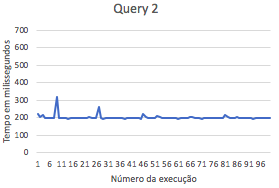
\includegraphics[scale=0.7]{Query2_Set}
    \caption{Resultados da implementação da query 2 com usersPostsSet}
    \label{figRotulo}
  \end{minipage}
 \hfill
   \begin{minipage}[b]{0.5\textwidth}
      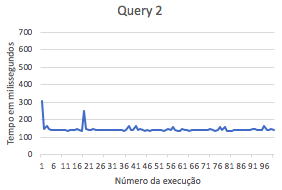
\includegraphics[scale=0.7]{Query2_List}
      \caption{Resultados da implementação da query 2 com usersPostsList}
      \label{figRotulo}
      \end{minipage}
    \end{figure}

    \vspace{0.4cm}

Conforme podemos observar a partir dos gráficos, a implementação da query 2 utilizando
uma TreeSet de usuários ordenada por ordem decrescente de número de posts,
é menos eficiente, já que em média leva 198,76 milissegundos(ms) a preencher
devidamente a TreeSet e a responder à query 2, ao passo que com uma lista,
o mesmo processo, leva em média 144,45 ms,o que equivale a um ganho de cerca de
50 ms, pelo que optamos pela implementação da query 2 descrita na secção Queries.

\section{Conclusões}
\label{sec:conclusao}

Face ao problema apresentado e analisando criticamente a solução proposta concluímos
que cumprimos todas as tarefas, conseguindo atingir os objetivos definidos. No decurso
do projeto socorremo-nos dos conhecimentos adquiridos nas unidades curriculares de
Algoritmos e Complexidade, Programação Orientada a Objetos, bem como Arquitetura de Computadores
de forma a equacionarmos a melhor solução para o problema apresentado, conseguindo
obter resultados bastante satisfatórios face ao que nos foi pedido. \par
Todavia, entendemos que há alguns aspetos da nossa solução que, eventualmente,
poderiam ser melhorados. Com efeito, infelizmente, não tivemos tempo para testar,
em termos de desempenho, todas as soluções possíveis e que pudessem fazer diferença
a nível de tempo em todas as queries.\par
Em suma, não obstante as potenciais melhorias que poderiam ser feitas no
programa, os testes por nós realizados, nas nossas máquinas, atingiram
um tempo de execução que consideramos bastante aceitável.



\end{document}
